\section{Numerical Results}
\label{sec:numres}
With the mathematical model now fully established, the implementation of this model is documented in Section \ref{subsec:impl}. From here Sections \ref{subsec:vv} verifies the model against exact dispersion relations for multiple modes in rectangular waveguides. Section \ref{subsec:circ_guides} performs an analysis of Dispersion characteristics in circular waveguides and addresses the advantages of using FEA for this task. Finally, Section \ref{subsec:rid_guides} compares the dispersion characteristics of the rectangular and ridged rectangular waveguides for multiple modes and discusses practical applications of ridged waveguides.

\subsection{Implementation}
\label{subsec:impl}
All meshes used in the following sections were generated using Coreform Cubit \cite{cubit} with a tutorial provided by \cite{rothlecnotes}. For the rectangular waveguide found in \ref{subsec:vv}, a WR-90, X-band waveguide with $a=0.02286$m and $b=0.01016$m was used \cite{everythingrf}. For the circular waveguide used in \ref{subsec:circ_guides}, a similarly sized circular waveguide of radius $r=0.01$m was used. In order to compare the non-ridged to the ridged waveguide the same WR-90, X-band waveguide was used in Section \ref{subsec:rid_guides} as in Section \ref{subsec:vv}; however, with two $0.0025\times0.0025$m notches cut out along the long edge. Example meshes of the later two geometries can be found in Figures \ref{fig:circular_guide}-\ref{fig:ridged_guide}. These meshes were generated using Coreform Cubit's \verb|TriAdvance| algorithm all containing $\approx2000$ nodes which is appropriate for the applications studied here. Coreform Cubit's \verb|nodeset| feature was used to create a set of all nodes on the boundaries of these geometries. This allows for $O(1)$ lookups of elements on the boundary which was utilized heavily when performing TM mode analysis. These meshes were saved into the ABAQUS \verb|.inp| ASCII format, which was chosen for its human readability which was invaluable during the development of this code.

\begin{figure}[h!]  
	\centering
	%the command within the [] sets the width of the figure, stability-condition is the jpg name
	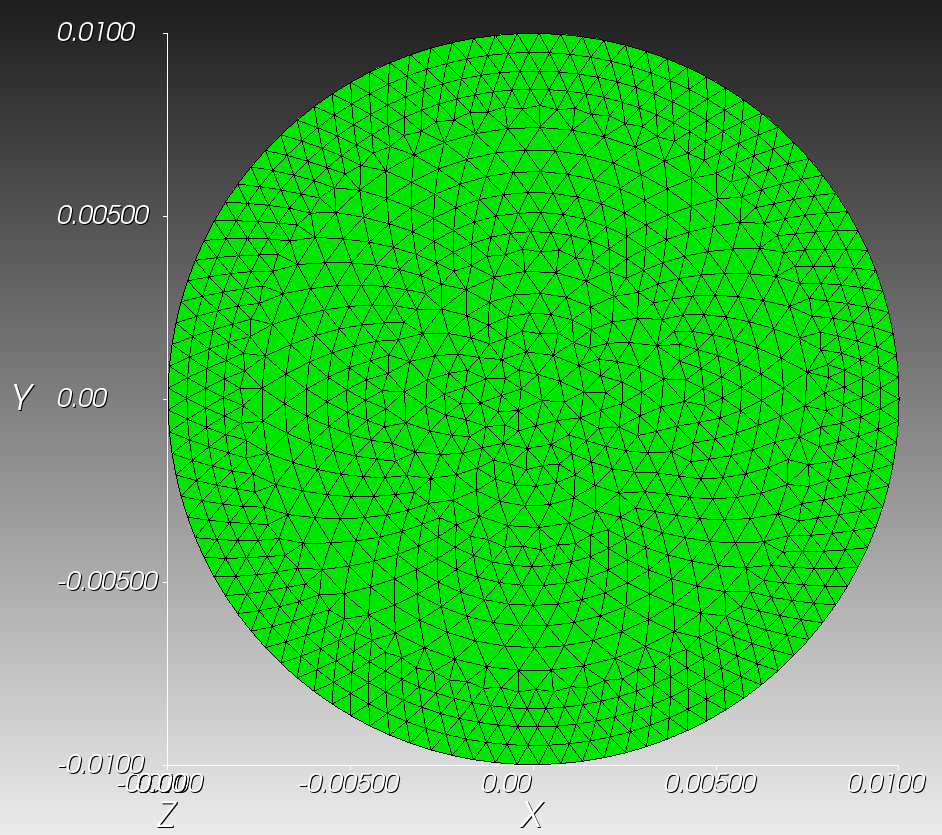
\includegraphics[width=\columnwidth]{circular_mesh.png} 
	\caption{Circular Waveguide Mesh used in Section \ref{subsec:circ_guides}}
	\label{fig:circular_guide}
\end{figure}

\begin{figure}[h!]  
	\centering
	%the command within the [] sets the width of the figure, stability-condition is the jpg name
	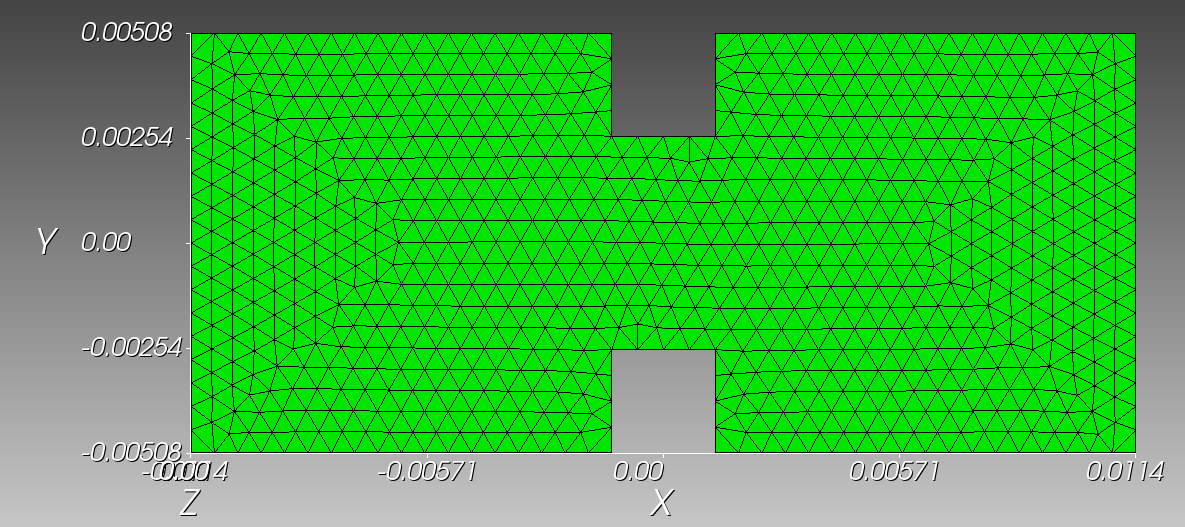
\includegraphics[width=\columnwidth]{ridged_mesh.png} 
	\caption{Ridged Rectangular Waveguide Mesh used in Section \ref{subsec:rid_guides}}
	\label{fig:ridged_guide}
\end{figure}

The mathematical model outlined in Section \ref{sec:mathmod} was implemented in Python for its general flexibility and existing numerical packages such as NumPy and SciPy which were used to solve the general eigenvalue problems established in (\ref{eq:te_eig}-\ref{eq:tm_eig}). In addition to these packages, the MeshIO package was used as it has a built in reader for \verb|.inp| files, allowing mesh data to be read in with ease. From this, all generated data was directly plotted using Matplotlib thereby eliminating the need to save any generated data to disk.

\subsection{Verification and Validation}
\label{subsec:vv}
Prior to performing any kind of `novel' analysis, the implemented model must first be benchmarked against analytic results. For this reason, the case of a WR-90, X-band waveguide with $a=0.02286$m and $b=0.01016$m is first considered \cite{everythingrf}. 

In this and all following sections the spatial distributions of TE modes will be plotted. Only one mode will be plotted per section as these are merely visual aids in comparison to the dispersion charts which will contain data from the first 3 TE and TM modes. The choice of the given TE mode is entirely arbitrary and was chosen for its post processing simplicity and to ensure adequate comparisons exist in the literature \cite{pozar2011microwave}. The $\mathrm{TE}_{11}$, $H_z$ field distribution can be found in Fig. \ref{fig:rect_prof}. 

\begin{figure}[h!]  
	\centering
	%the command within the [] sets the width of the figure, stability-condition is the jpg name
	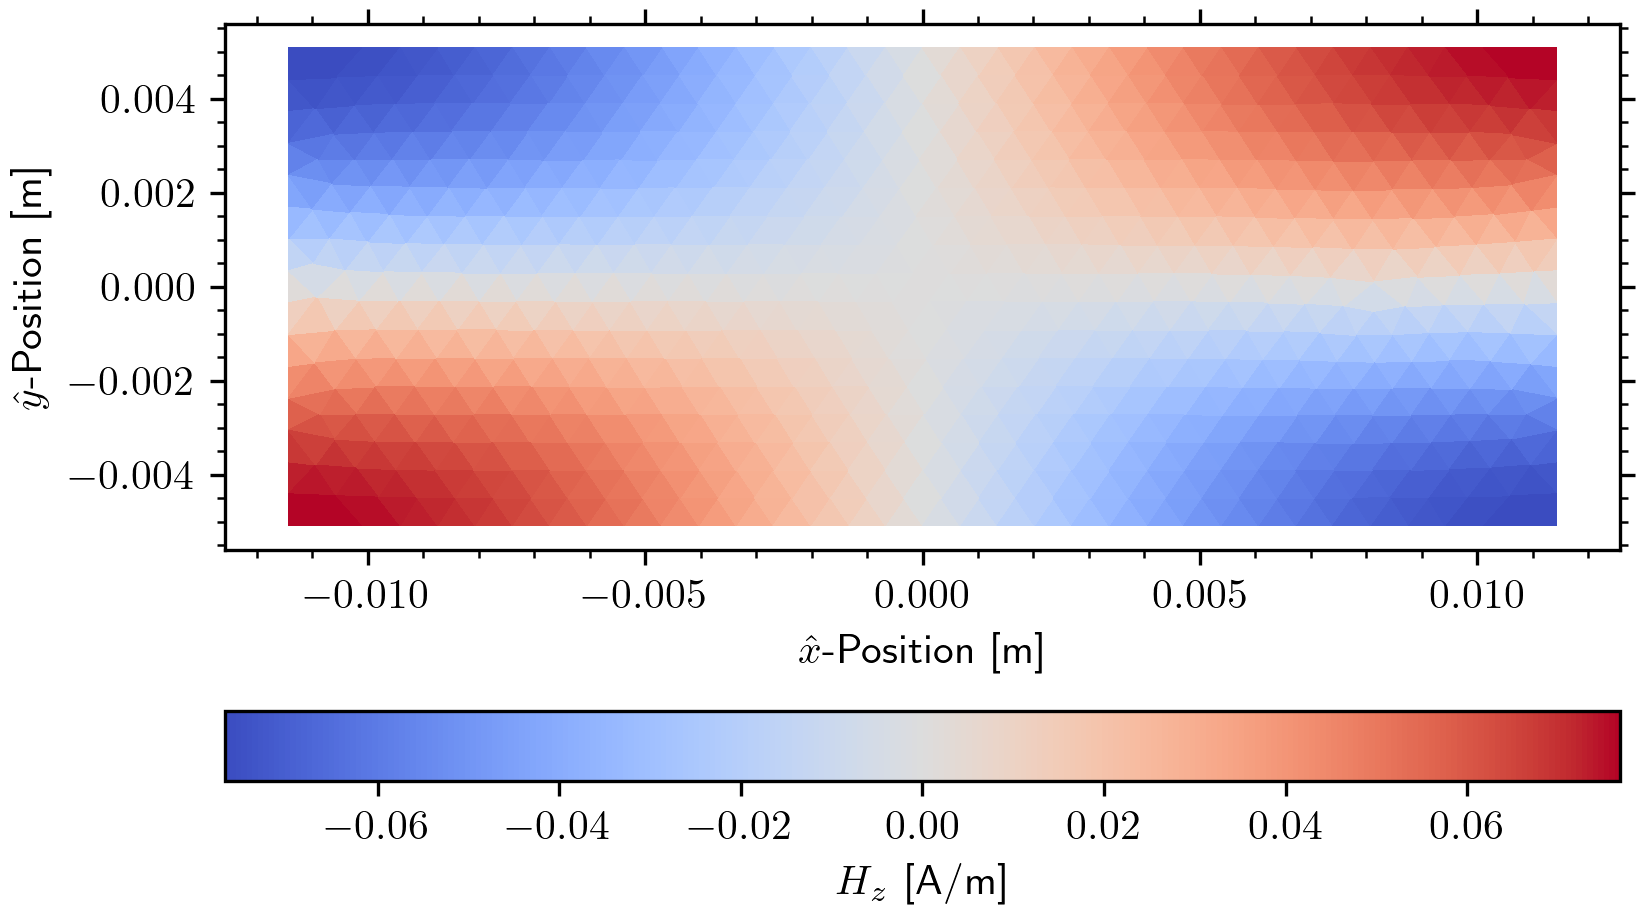
\includegraphics[width=\columnwidth]{te11_rect.png} 
	\caption{$\mathrm{TE_{11}}$, $H_z$ Field Distribution in a Rectangular WR-90, X-band Waveguide}
	\label{fig:rect_prof}
\end{figure}

As seen in Fig. \ref{fig:rect_prof} the $\mathrm{TE_{11}}$, $H_z$ field profile matches that of the $\mathrm{TE}_{11}$ found in the literature \cite{pozar2011microwave} thus confirming its accuracy in recreating spatial field profiles. The $\mathrm{TE}_{10}$ and $\mathrm{TE}_{21}$ modes profiles were also vetted, however are not shown to reduce clutter.

Next, a dispersion plot of the first three TE and TM modes in this waveguide is constructed. To benchmark to theory, the following analytic cutoff wave number is used:
\begin{align}
    k_c=\sqrt{\left(\frac{m\pi}{a}\right)^2+\left(\frac{n\pi}{b}\right)^2},
\end{align}
where $m$ and $n$ are the corresponding mode propagation numbers. From this, the first three, unique, and nonzero simulated cutoff wave numbers from both the TE and TM modes were used to create the dispersion plot in Fig. \ref{fig:rect_disp}.

\begin{figure}[h!]  
	\centering
	%the command within the [] sets the width of the figure, stability-condition is the jpg name
	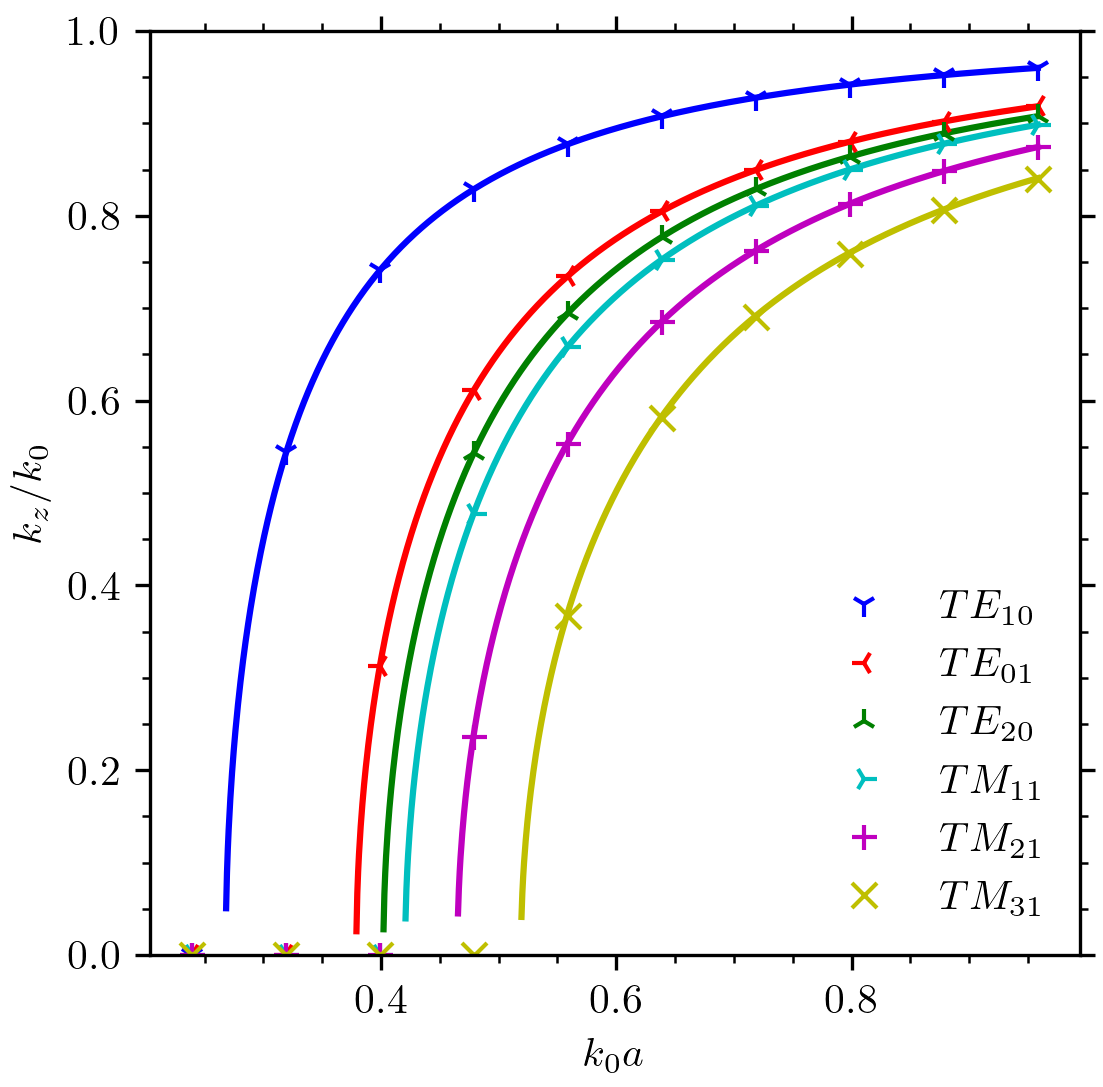
\includegraphics[width=\columnwidth]{rec_waveguide_disp.png} 
	\caption{Dispersion Plots of First Three TE and TM Modes in Rectangular WR-90, X-band Waveguide with Solid Lines as Analytical Results and Corresponding Markers as Simulated Results}
	\label{fig:rect_disp}
\end{figure}

As seen in Fig. \ref{fig:rect_disp}, the dispersion relations predicted by the implemented model match that predicted by theory excellently. Additionally, this demonstrates that the choice of using $\approx2000$ nodes to represent these geometries is more than sufficient to ensure convergence on the true solution. With this, more sophisticated waveguides can now be investigated knowing that the underlying mathematical model is sound.


\subsection{Circular Waveguides}
\label{subsec:circ_guides}
With the model successfully validated against the analytic results of a rectangular waveguide, a circular waveguide of radius $r=0.01$m is now assessed. One last visual verification step is performed by comparing the field profiles of the $\mathrm{TE}_{01}$ and $\mathrm{TE}_{11}$ modes generated by the model to that of the analytic profiles found in literature. The simulated $\mathrm{TE}_{01}$ $H_z$ profile can be found in Fig. \ref{fig:circ_prof}.

\begin{figure}[h!]  
	\centering
	%the command within the [] sets the width of the figure, stability-condition is the jpg name
	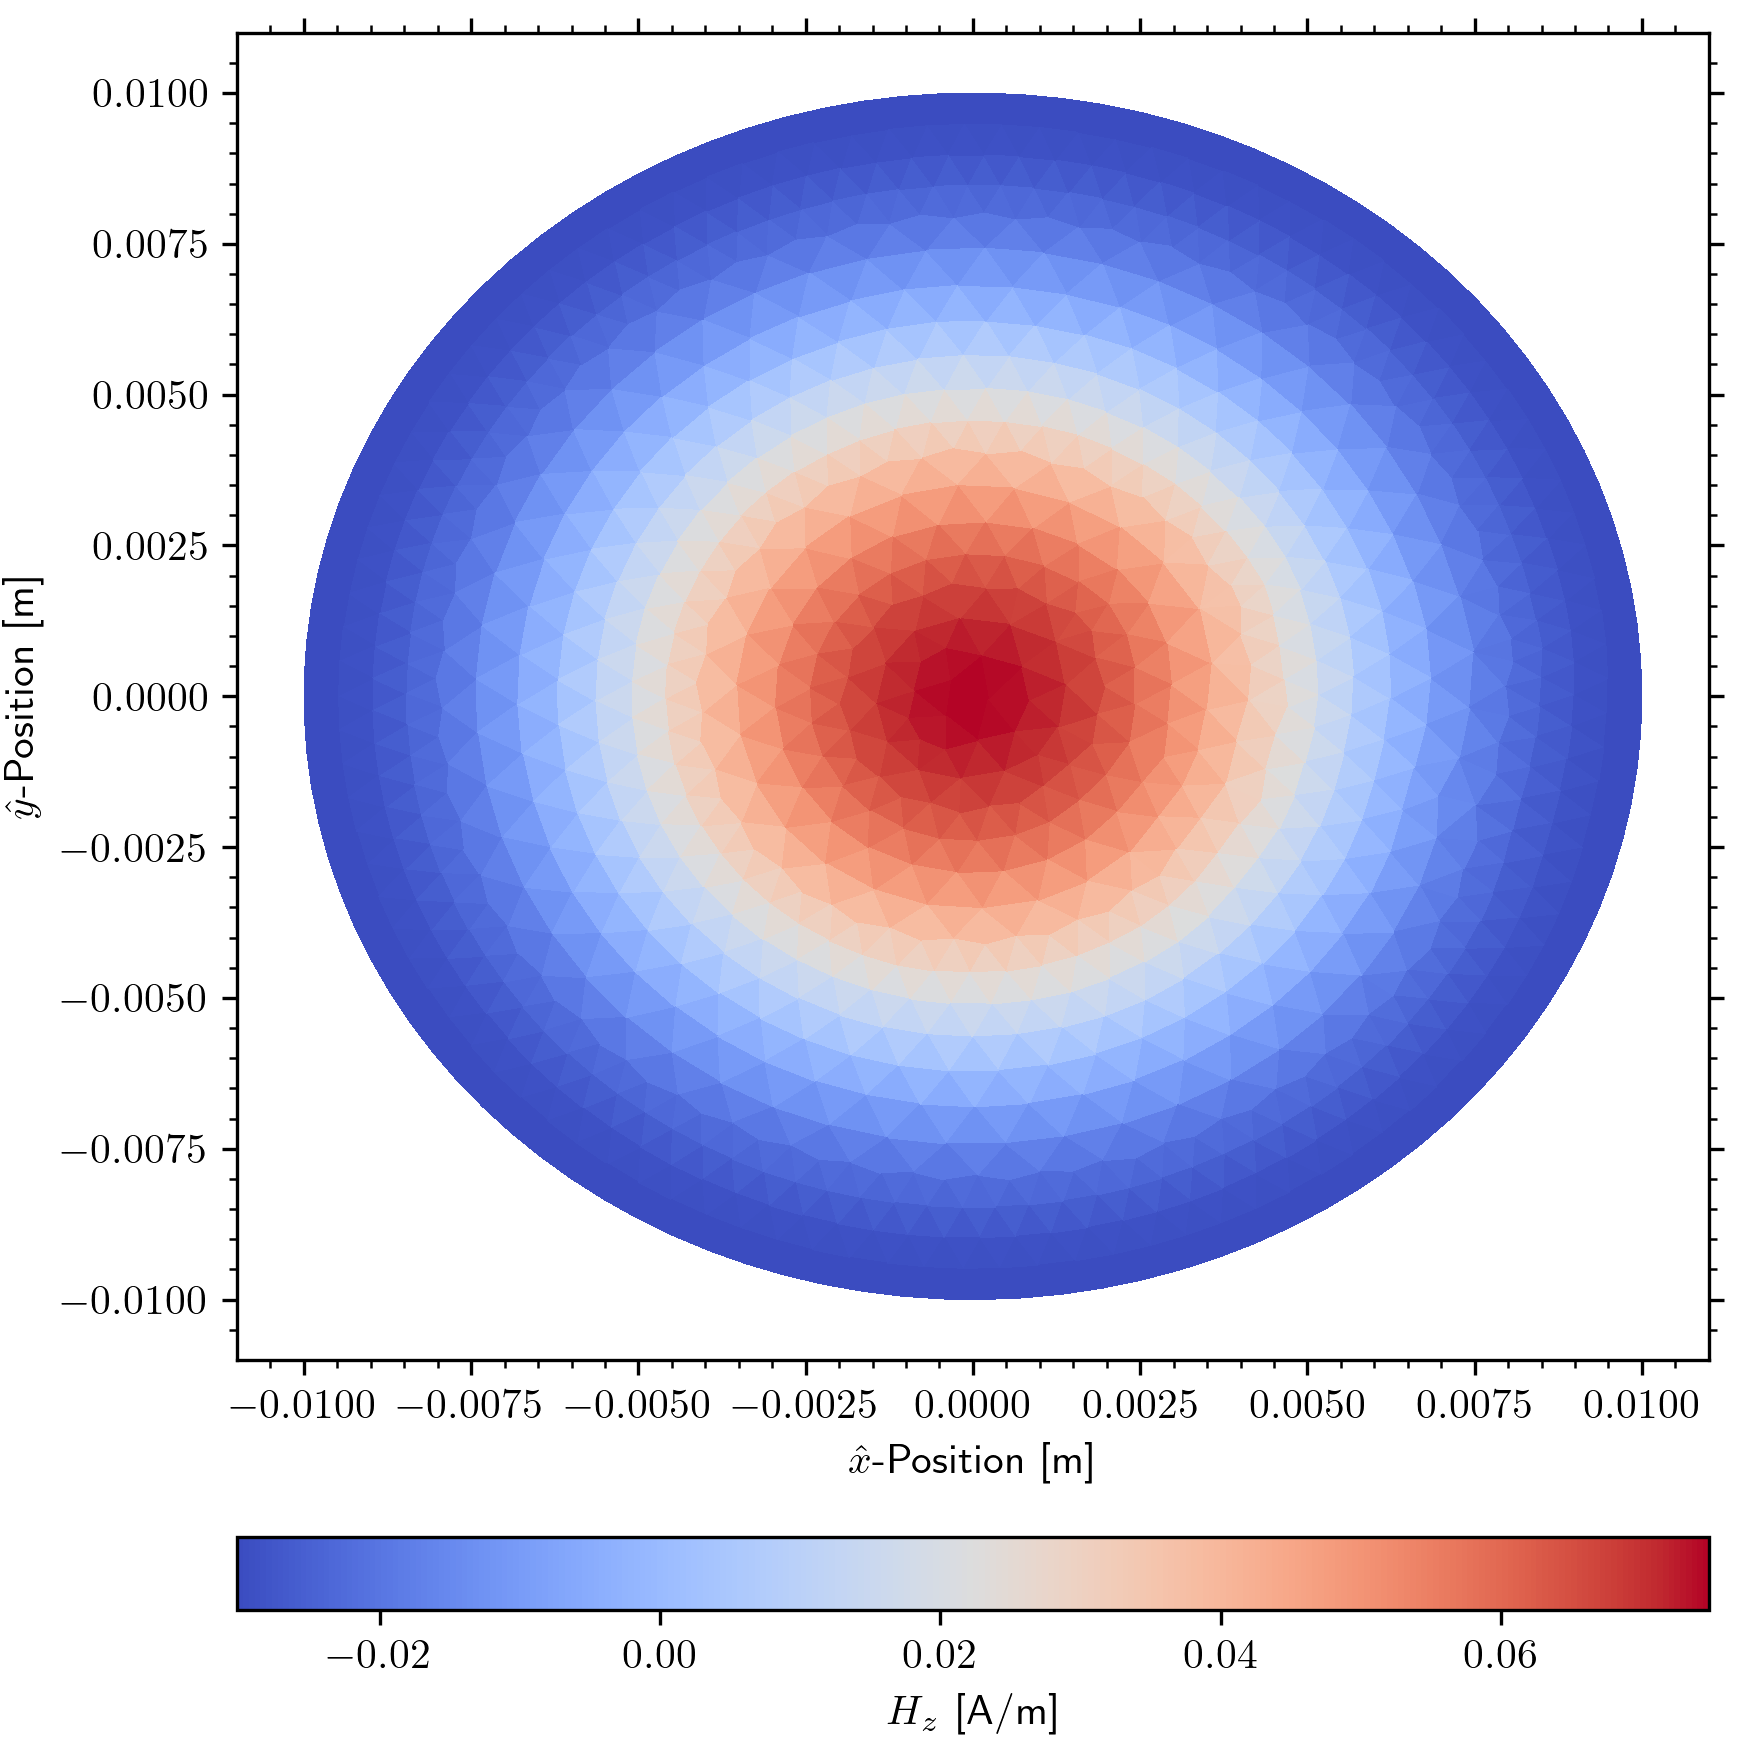
\includegraphics[width=\columnwidth]{te01_circ.png} 
	\caption{$\mathrm{TE_{01}}$, $H_z$ Field Distribution in a Circular Waveguide with $r=0.01$m}
	\label{fig:circ_prof}
\end{figure}

As seen in Fig. \ref{fig:circ_prof}, the $H_z$ profile matches that found in the literature \cite{pozar2011microwave}, thereby providing additional validation for the implemented numerical model. These field plots also highlight one of the main strengths of FEM; which is its ability to work with unstructured grids out of the box. Modeling a similar profile using a finite difference method would result in egregious stair-stepping error if performed in Cartesian coordinates, or would require a special derivation in polar or cylindrical coordinates potentially limiting the model's usefulness. On the other hand, FEA is able to handle these curved geometries using unstructured grids with relative ease. 

From here a similar analysis to that of Fig. \ref{fig:rect_disp} is performed for circular waveguides. Traditionally, producing such plots would require tables containing roots of the Bessel function of the first kind $p_{nm}$ and it's derivative $p^{'}_{nm}$ which are used to determine the cutoff wave numbers as
\begin{align}
	k_c = \frac{p^{'}_{nm}}{r},
\end{align}
and
\begin{align}
	k_c = \frac{p_{nm}}{r}
\end{align}
respectfully for the TE and TM modes \cite{pozar2011microwave}. Using the above FEM, we are able to directly calculate the dispersion relations for any circular waveguide without the use of the roots of a Bessel function or its derivative. The simulated dispersion relations can be found in Fig. \ref{fig:circ_disp}.

\begin{figure}[h!]  
	\centering
	%the command within the [] sets the width of the figure, stability-condition is the jpg name
	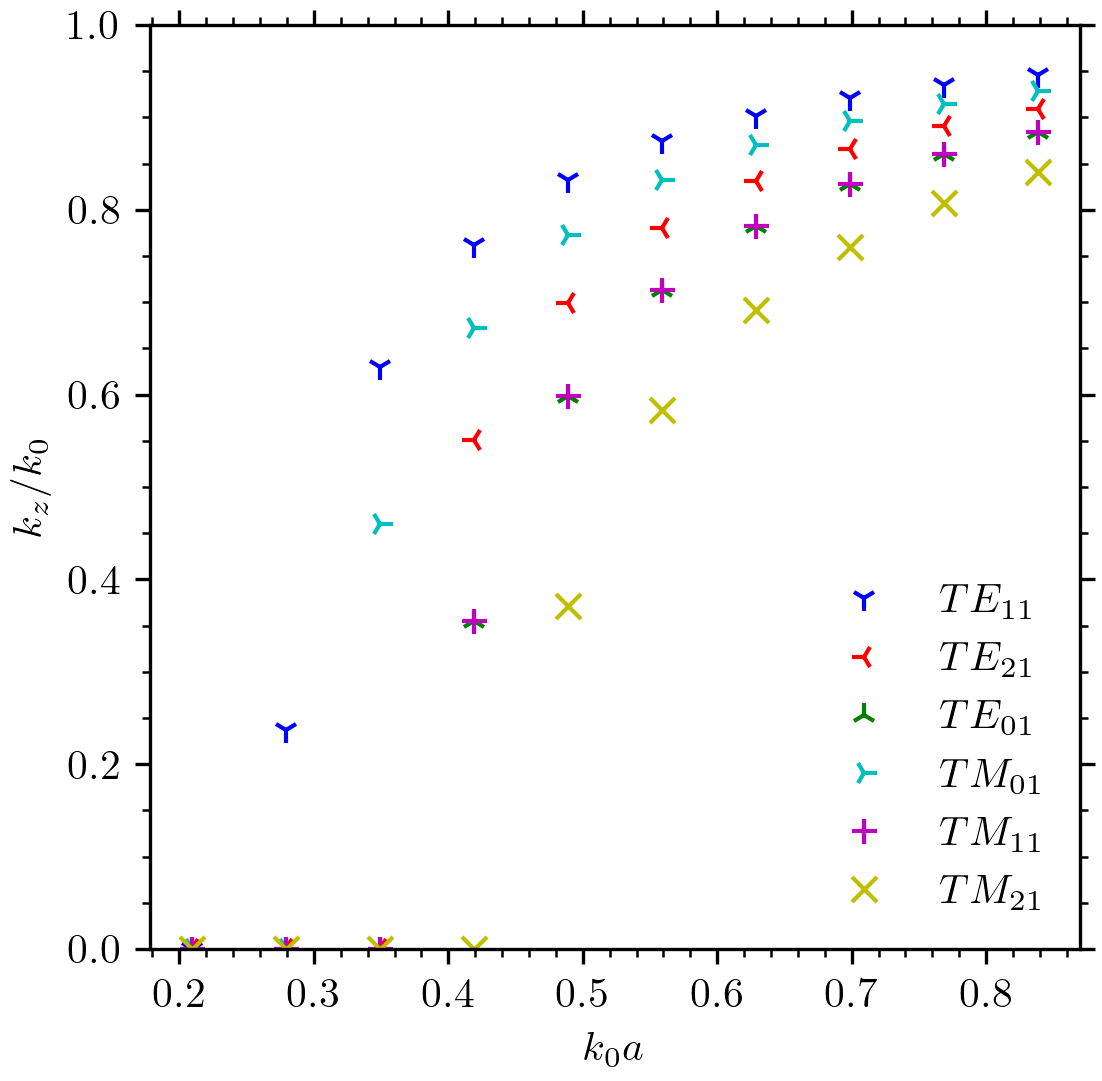
\includegraphics[width=\columnwidth]{circ_waveguide.png} 
	\caption{Dispersion Plots of First Three TE and TM Modes in a Circular Waveguide with $r=0.01$m}
	\label{fig:circ_disp}
\end{figure}

As seen in Fig. \ref{fig:circ_disp}, the bandwidth between individual propagation modes in a circular waveguide is much less than that of rectangular waveguides as shown in Fig. \ref{fig:rect_disp}. This is perhaps most notable between the $\mathrm{TE}_{11}$ dominant mode and the next $\mathrm{TM}_{01}$ mode, which is rather small. This is well documented in the literature \cite{cadencecircular} and is one of the main factors limiting circular waveguides from being used in wide-band applications. Finally, FEA was able to successfully predict the equivalence of the cutoff wave number for the  $\mathrm{TE}_{01}$ and $\mathrm{TM}_{11}$ modes which is well documented in the literature \cite{pozar2011microwave} thereby providing one last verification step prior to considering ridged rectangular waveguides.

\subsection{Comparison of Ridged and Non-Ridged Waveguides}
\label{subsec:rid_guides}
With all validation steps completed, a comparison of a standard WR-90, X-band waveguide to that of a double ridged WR-90, X-band waveguide is now provided. As seen in Fig. \ref{fig:ridged_guide}, ridges are of size $0.0025\times0.0025$m and are placed at the centerline of the waveguide. Similarly to Section \ref{subsec:vv},the $H_z$ field profile of the $\mathrm{TE_{11}}$ mode is assessed as shown in Fig. \ref{fig:rid_prof}.

\begin{figure}[h!]  
	\centering
	%the command within the [] sets the width of the figure, stability-condition is the jpg name
	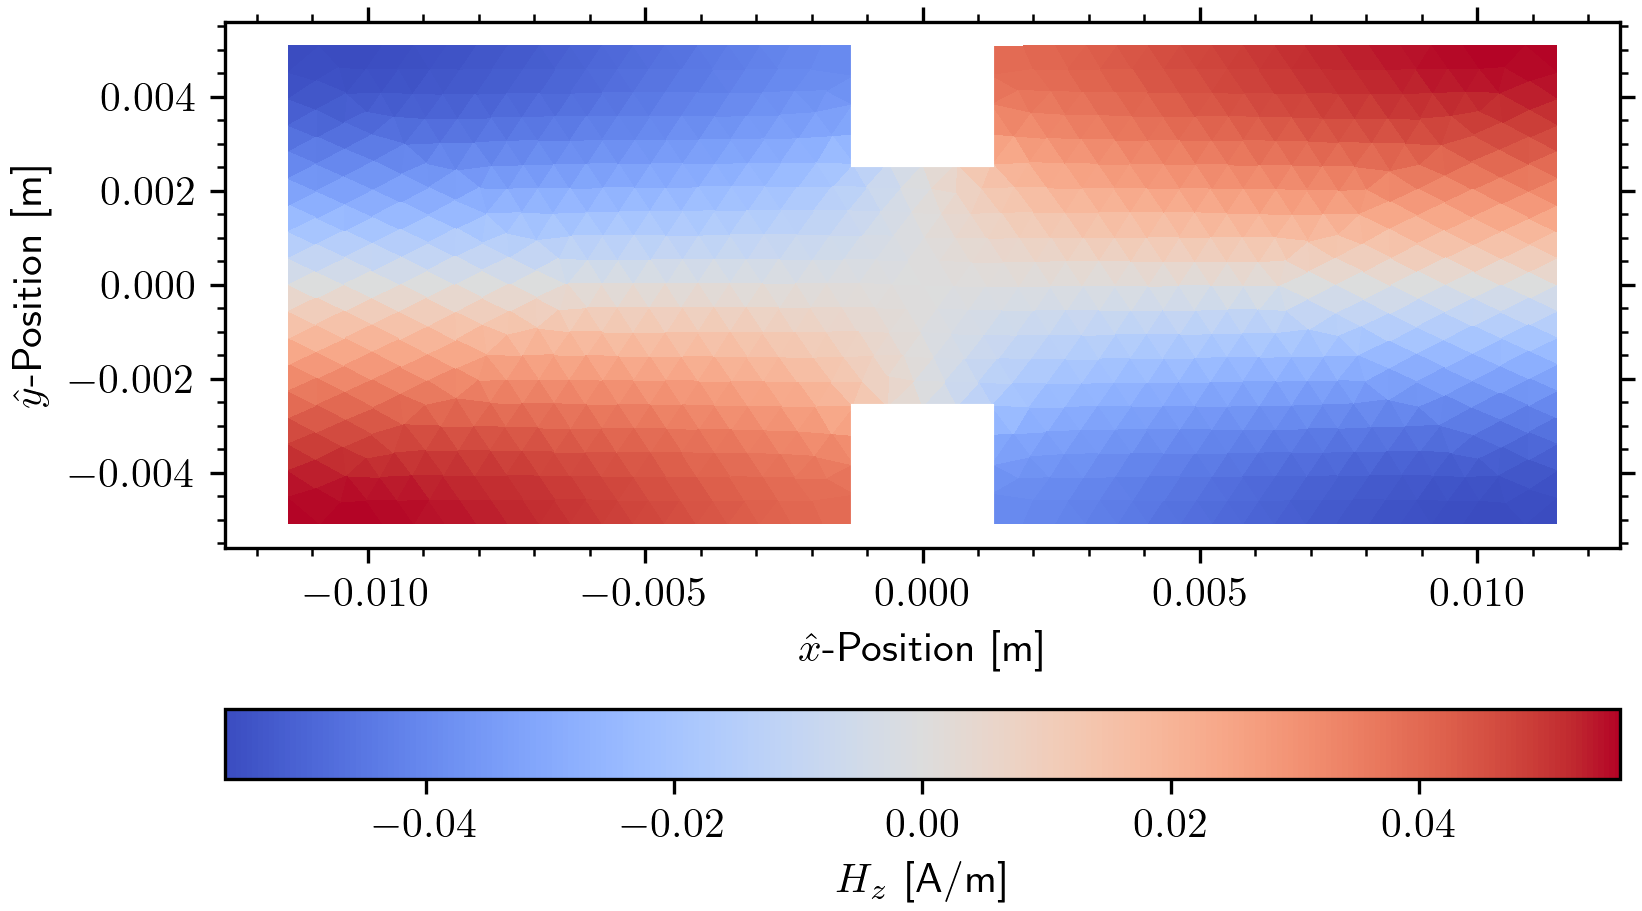
\includegraphics[width=\columnwidth]{te11_rid.png} 
	\caption{$\mathrm{TE_{11}}$, $H_z$ Field Distribution in a Ridged Rectangular WR-90, X-band Waveguide}
	\label{fig:rid_prof}
\end{figure}

As seen in Fig. \ref{fig:rid_prof} the field profile is nearly identical to that of the non-ridged WR-90 waveguide shown in Fig. \ref{fig:rect_prof}. This is expected as the propagation mode is identical despite the introduction of ridges. To demonstrate differences, a dispersion plot for this ridged waveguide is provided. To highlight discrepancies between the ridged and base waveguides, the theoretical base dispersion curves are plotted as solid lines, and the corresponding simulated data for the same modes as markers. Said plot can be found in Fig. \ref{fig:rid_disp}.

\begin{figure}[h!]  
	\centering
	%the command within the [] sets the width of the figure, stability-condition is the jpg name
	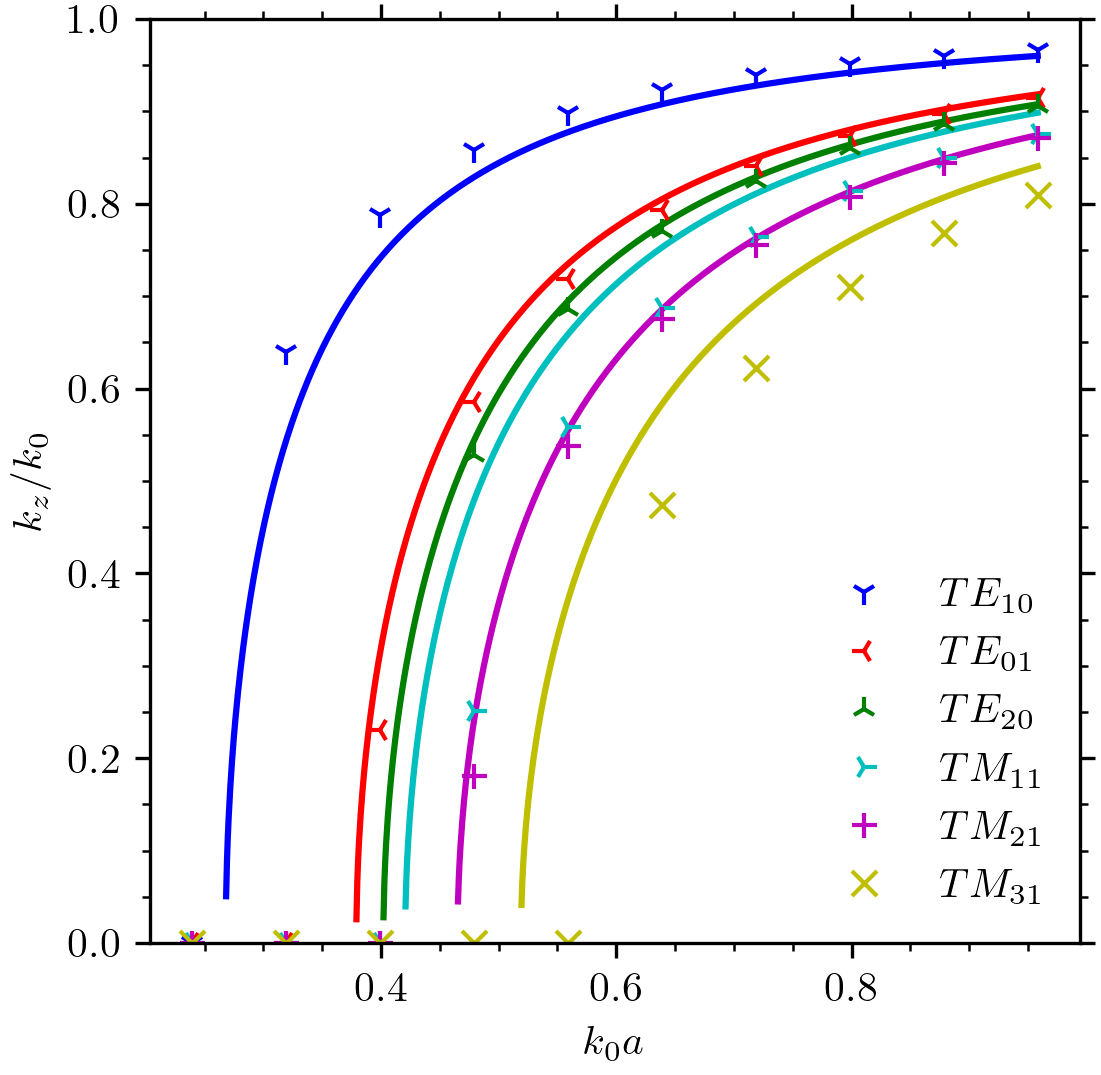
\includegraphics[width=\columnwidth]{ridged_waveguide_w_comp} 
	\caption{$\mathrm{TE_{11}}$, $H_z$ Field Distribution in a Ridged Rectangular WR-90, X-band Waveguide with Solid Lines as the Theoretical Dispersion Relation for Base Waveguide and Corresponding Markers as Simulated Dispersion Relation for Ridged Waveguide}
	\label{fig:rid_disp}
\end{figure}

It is clear from Fig. \ref{fig:rid_disp} that the cutoff wave number of the dominant $\mathrm{TE}_{10}$ mode is less than that of the rectangular waveguide in alignment with the theory \cite{pozar2011microwave}. In addition to this, all fields with cutoff wave numbers greater than the dominant mode all experience an increase in cutoff wave number within the ridged waveguide. These phenomenon can all be explained via field buckling caused by the inclusion of ridges. To demonstrate this, the field profiles of the dominant $\mathrm{TE}_{10}$ modes for both the base and ridged waveguides are plotted which can be found in Figs. \ref{fig:rec_te10}-\ref{fig:rid_te10}.

\begin{figure}[h!]  
	\centering
	%the command within the [] sets the width of the figure, stability-condition is the jpg name
	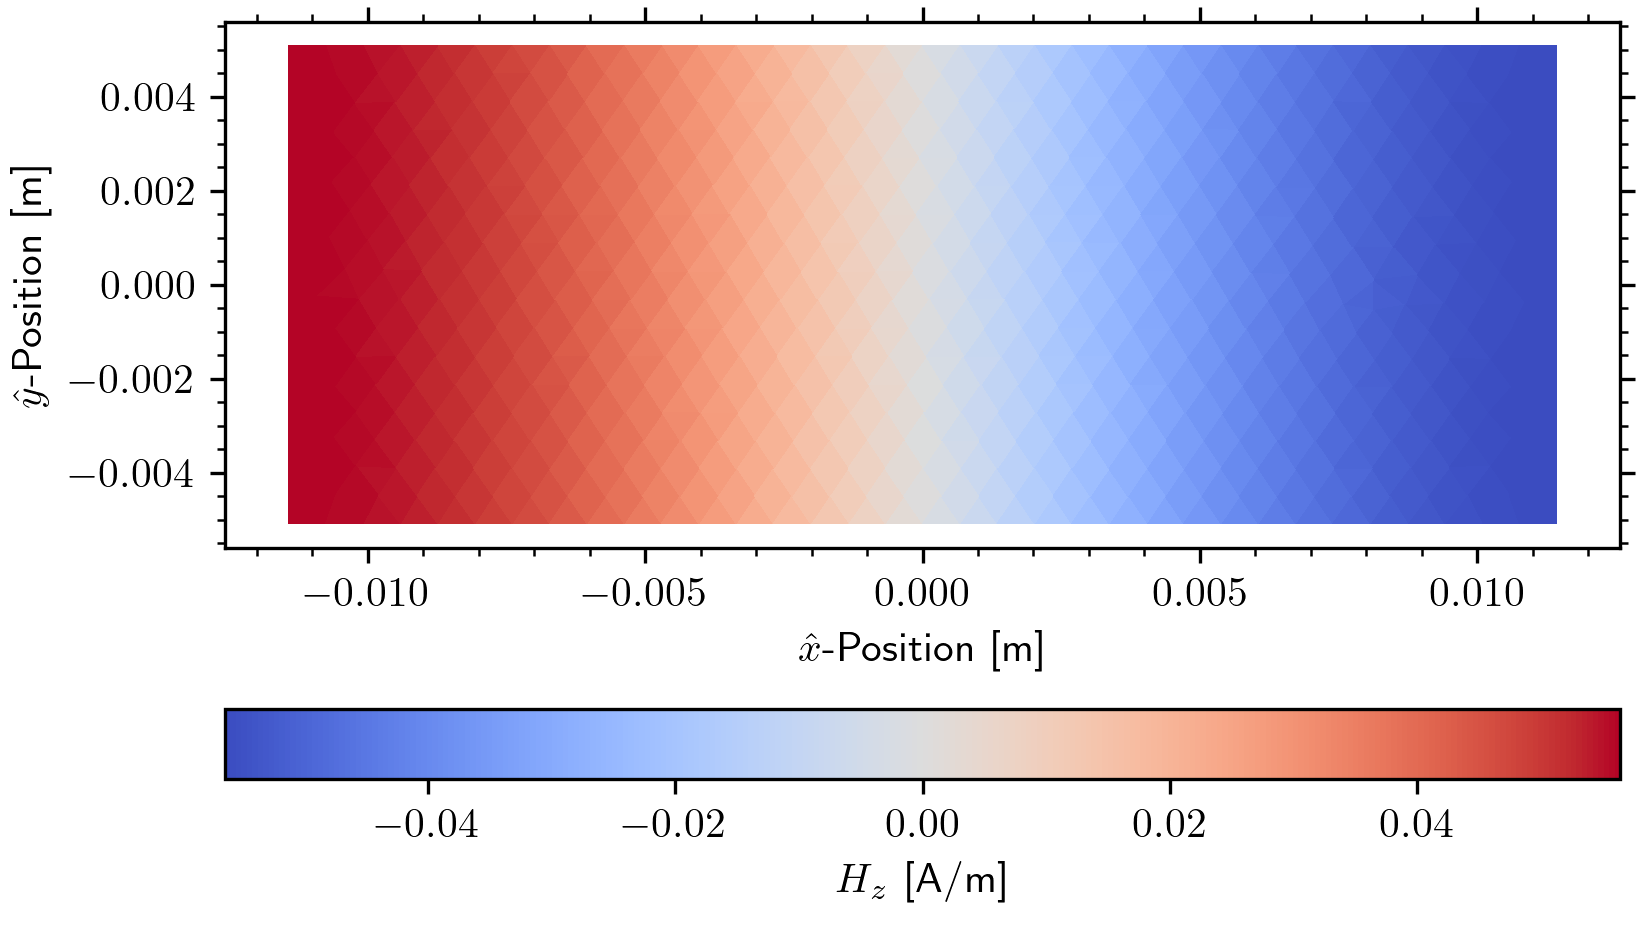
\includegraphics[width=\columnwidth]{te10_rect.png} 
	\caption{Dominant $\mathrm{TE_{10}}$, $H_z$ Field Distribution in a Rectangular WR-90, X-band Waveguide}
	\label{fig:rec_te10}
\end{figure}

\begin{figure}[h!]  
	\centering
	%the command within the [] sets the width of the figure, stability-condition is the jpg name
	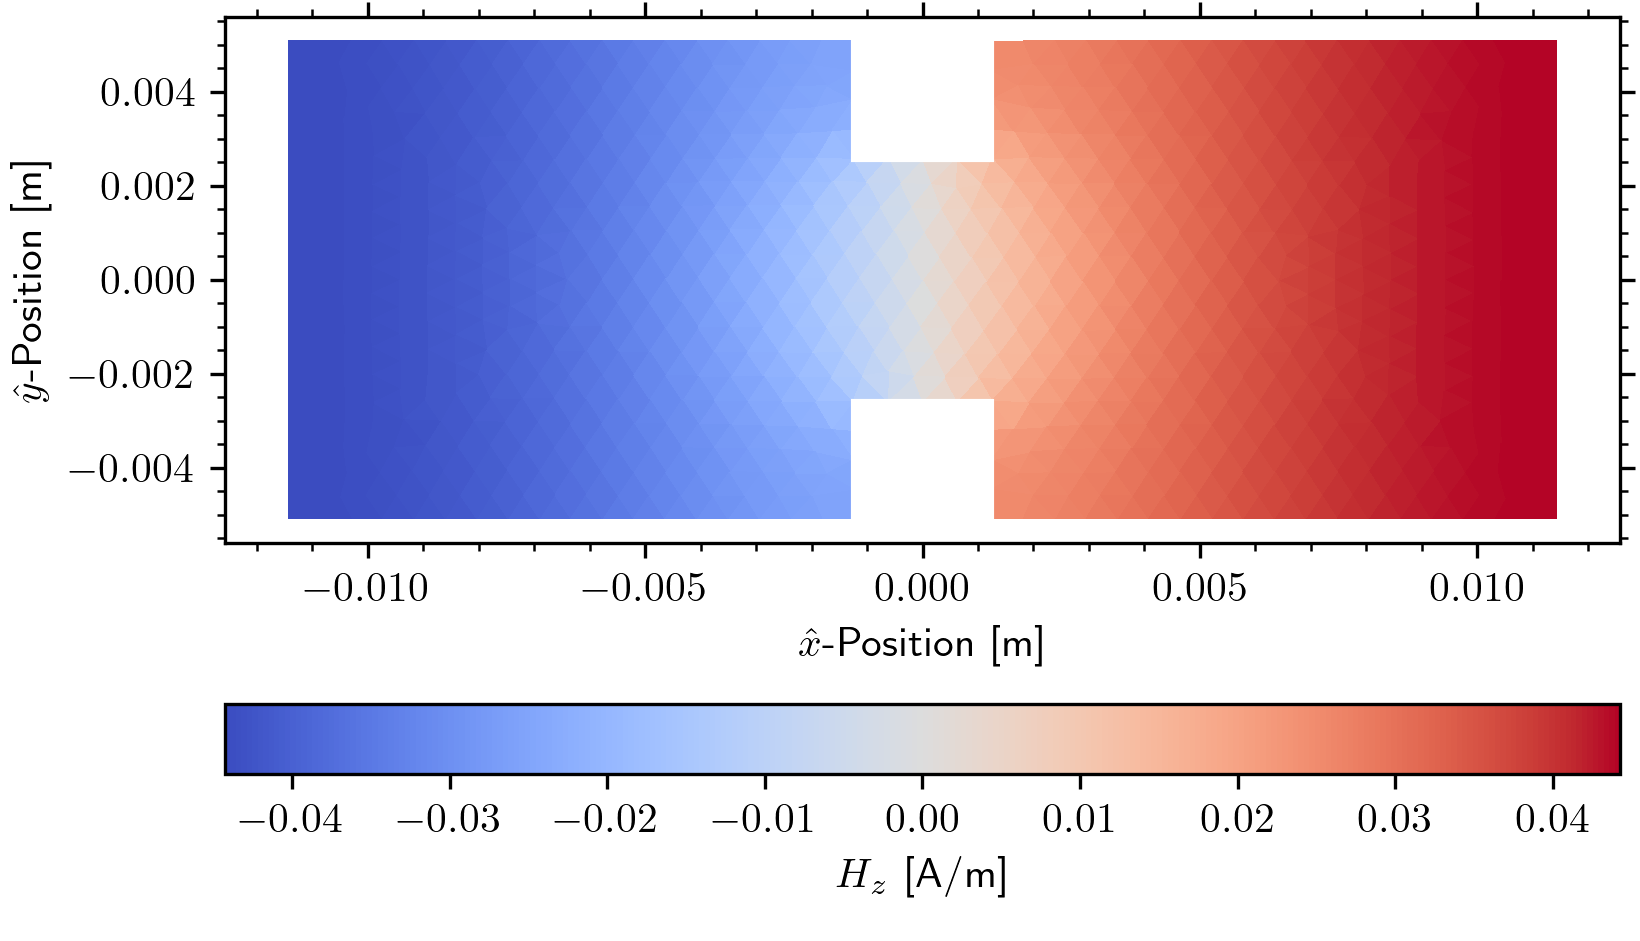
\includegraphics[width=\columnwidth]{te10_ridged.png} 
	\caption{Dominant $\mathrm{TE_{10}}$, $H_z$ Field Distribution in a Ridged Rectangular WR-90, X-band Waveguide}
	\label{fig:rid_te10}
\end{figure}

Fig. \ref{fig:rec_te10} shows that in the base waveguide there are two distinct regions within the $\mathrm{TE}_{10}$, $H_z$ field profile. In the case of the ridged waveguide, the ridges align with the gap between these field regions allowing for the same field profile to be achieved at lower frequencies, thus resulting in the lowering of the cutoff wave number. In other words, the inclusion of ridges facilitates a lower overall field buckling for this propagation mode. In contrast to this, higher order modes such as the $\mathrm{TE}_{11}$ mode found in Fig. \ref{fig:rid_prof} require increased buckling in order to satisfy the boundary conditions of (\ref{eq:diriclet_tm}-\ref{eq:neumann_te}) to achieve the same field profile. This increased field buckling directly corresponds to an increase in the minimum cutoff wave number, and corresponding frequency content, to recreate these higher-order, more complex, propagation modes. For this reason, ridged waveguides offer superior bandwidth for the dominant modes making them superior for transmitting high-bandwidth signals.   
